\section{Problem 1} \label{sec:mm5_Pb1}
\textit{How does the packet length affect the thresholds for adaptive modulation in case of uncoded modulation?}

The length of the packets might affect the way how we choose the thresholds to go up in modulation in an adaptive modulation scheme. When we have a long packet, we want to choose a threshold in a more cautious way i.e. it is wanted to go up in modulation only if we are pretty sure that a good channel is present. This is done in this way because loosing a long packet hurts the system more than loosing a small one.

On the other hand, when we are using short packets, the thresholds to go up in modulation can be chosen in a more aggressive way. Loosing some small packets due to this miscalculations of the channel conditions might, on average, be less expensive that the increased rates that can be earned by going up in modulation fast.

For going down in the chosen modulation, the thresholds are chosen the other way around i.e. for long packets we go down in modulation faster than if we are using short packets. These ideas are illustrated on \figref{fig:thresholds_packet_size}


\begin{figure}[!h]
  \centering
  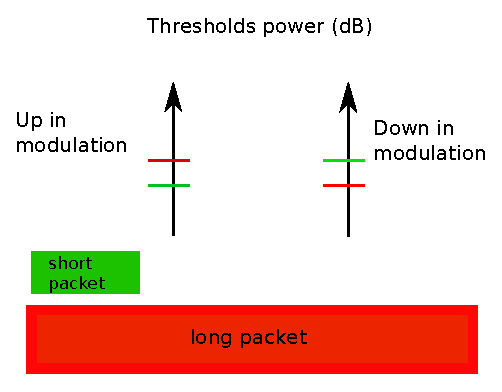
\includegraphics[width=8cm]{figures/thresholds_packet_size.eps}
  \caption{Relationship between packet length and thresholds in adaptive modulation schemes}
  \label{fig:thresholds_packet_size}
\end{figure}